\documentclass[12pt,a4paper]{report}
\usepackage[utf8]{inputenc}
\usepackage{amsmath}
\usepackage{amsfonts}
\usepackage{amssymb}
\usepackage{graphicx}
\usepackage[noadjust]{cite}
\usepackage{url}
%\usepackage{lipsum}
\usepackage{filecontents}
%\author{Mohammed Saifuddin}
\author{
	\\Mohammed Saifuddin\\
	\texttt{1640272|4CMS}
	\and
	\\Mohammed Sameeruddin\\
	\texttt{1640273|4CMS}
	\and
	\\Manish Chhetri\\
	\texttt{1640205|4CMS}
	\and
	\\Shashank Sekhar\\
	\texttt{1640253|4CMS}
}

\title{\textbf{\huge{Traffic Model and Simulation}}}
\date{}

\begin{filecontents*}{bibo.bib}
	@inbook{mc,
		author = {William L Brogan},
		title = {Modern Control Theory},
		publisher = {Pearson},
		year = {2011},
		edition = {3}
	}

	@online{lo,
		author = {Benjamin Seibold},
		title = {A Mathematical Introduction to Traffic Flow Theory},
		year = {2015},
		note = {\url{http://helper.ipam.ucla.edu/publications/tratut/tratut_12985.pdf}},
		organization = {Institute for Pure and Applied Mathematics}
	}

	@PhdThesis{kw,
		author = {Wenlong Jin},
		title = {Kinematic Wave Models of Network Vehicular Traffic},
		school = {University of California},
		year = {2003},
		month = {September},
		note = {\url{http://www.its.uci.edu/~wjin/publications/jin2003dissertation.pdf}}
	}

	@online{tf,
		title = {Traffic Flow},
		note = {\url{https://en.wikipedia.org/wiki/Traffic_flow}}
	}

	@online{rp,
		title = {Riemann problem},
		note = {\url{https://en.wikipedia.org/wiki/Riemann_problem}}
	}
\end{filecontents*}

\begin{document}
	\begin{titlepage}
		\centering
		
\includegraphics[width=1\textwidth]{logo.jpg} \par\vspace{1.5cm}
		{\scshape\huge CHRIST\\\large{(deemed to be university)} \par}
		\vspace{1cm}
		{\LARGE Department of Mathematics \par}
		\vspace{1.5cm}
		{\scshape\huge \textbf{Traffic Model and Simulation} \par}
		\vspace{2cm}
		\vfill
		{\large \today\par}
	\end{titlepage}
	
	\maketitle
	\tableofcontents
	
	\begin{abstract}
		\addcontentsline{toc}{chapter}{\textbf{Abstract}}
		This dissertation ponders on how the problem of traffic can be viewed mathematically and what is the underlying math behind this ubiquitous problem. We have a simple simulation to explain the relationship of density, speed and flow of vehicles. This quest centered mainly on density and flow of vehicles, which are governed by mathematics. We have implemented Kinematic Wave Model of traffic, that relates the movement of vehicles as waves and calculates the fluctuations of density values. Simulations were devised using a Python tool called VPython, which is computer framework in model building.
	\end{abstract}
	
	\section*{Introduction}
	\addcontentsline{toc}{chapter}{\textbf{Introduction}}
	Mathematical models are the functions or systems that uses mathematical concepts and principles to solve real world problems. A bridge between real world and mathematical theory [1]. These are natural methods or different perspectives of looking into a problem to the core. When the problem intensity catapults then these tend to be virtually necessary. These can be the approaches that can either be implicit or explicit to sort the issue(s).
	\subsection*{Traffic model}
	\addcontentsline{toc}{section}{\text{Traffic model}}
	Traffic model is a function which appertains the movement of vehicles to drivers behavior, vehicle type, weather conditions and traffic signals. These models are subject to both space and time limitations i.e., initial traffic conditions and boundary conditions. Movement of the vehicle is represented by its position at any time i.e., trajectory from which the speed and acceleration rate can be obtained [].
	\begin{figure}[hbtp]
		\centering
		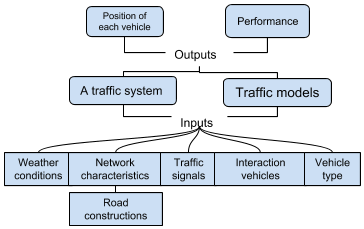
\includegraphics[scale=1]{some.png}
		\caption{Traffic Model}
	\end{figure}
	This traffic models are stringently calibrated and validated. Calibration is tuning parameters so that it acts closely to real traffic, whereas Validation is relative observation of results obtained by model and real traffic.
	\subsection*{Traffic congestion}
	\addcontentsline{toc}{section}{\text{Traffic congestion}}
	This is a phenomenon of vehicular queuing. Congestion occurs when traffic demand is great enough resulting slower mode of transportation. As demand increases incessantly reaching the capacity of road, extreme traffic sets in. When vehicles are utterly still for some period of time, this is known as traffic jam.
	\par Traffic congestions are of two types, recurrent and non-recurrent. Recurrent congestions are caused by limited physical infrastructure, increase in travel demand and toll booths. Non-recurrent congestions occur when there are any collateral damages like accidents and random unfavorable behavior of whether.
	\subsection*{Traffic flow}
	\addcontentsline{toc}{section}{\text{Traffic flow}}
	Traffic flow is the number of vehicles passing a reference point per unit of time. In mathematics, it is the study of interactions between travellers and road infrastructure. This flow is analogically assumed to be a wave slowly propagating forward [2].
	
	\section*{Traffic simulation and model}
	\addcontentsline{toc}{chapter}{\textbf{Traffic simulation and model}}
	As traffic emergence is random and unpredictable, we programmed a computational simulation that has this piquant feature of being random. Apart from that, we have a locomotory character that shows the variability of its speed depending on the density.
	\subsection*{Simulation}
	\addcontentsline{toc}{section}{\text{Simulation}}
	Any simulation is a computational mathematics that bounds to certain instruction to carry on. Our simulation has got three phases,
	\begin{enumerate}
		\item \textbf{Free phase}: This is indicated as green path, where in the locomotory character swiftly moves without any obstacles or congestion.
		\item \textbf{Moderate phase}: A yellow path indicates that the locomotory character is exhibiting moderate flow. This is a phase where there are few obstacles or congestion on road.
		\item \textbf{Dense phase}: This is phase where a vehicle hardly performs locomotion. This is called as traffic in the simulation.
	\end{enumerate}
	We have an interactive graphical representation that scales the density values by the time. Our simulation is not a wave though we practiced kinematic wave model. It is a Density flow simulation.
	\subsubsection*{Drawbacks of the simulation}
	\addcontentsline{toc}{subsection}{\text{Drawbacks of the simulation}}
	\begin{itemize}
		\item[$\bullet$] We considered only one locomotory character to emulate the traffic conditions centering to the concepts of density.
		\item[$\bullet$] This emulation deals only with density and flow of vehicles. Hence there is an inevitable plausibility of being unreliable.
	\end{itemize}
	\subsection*{Model}
	\addcontentsline{toc}{section}{\text{Model}}
	We implemented Kinematic Wave Model. This is a macroscopic traffic flow model that frame relationships among speed, density and flow of vehicles. This traffic stream flow was mainly brought under the assumption of a fluid stream. This was first implemented by Lighthill and Whitham in 1955. Later Richards posited the idea of shock-waves on the highway.
	\subsubsection*{Speed}
	\addcontentsline{toc}{subsection}{\text{Speed}}
	Speed is distance covered over unit time. It is unlikely and impractical to calculate or record the speed of every vehicle, so the best practice of tracking the speed is to consider average speed of sampling vehicles over a period of time [2].
	$$S = D/T$$
	\subsubsection*{Time mean speed}
	\addcontentsline{toc}{subsection}{\text{Time mean speed}}
	Time mean speed is measured at a reference point on the roadway over a period of time. Loop detectors are leveraged to measure the speed [2].
	$$v_t = (1/m)\sum_{i=1}^{m}v_i$$
	where $m$ represents the number of vehicles passing the fixed point and $v_i$ is the speed of the $i$th value.
	\subsubsection*{Space mean speed}
	\addcontentsline{toc}{subsection}{\text{Space mean speed}}
	Space mean speed is measured over the whole roadway segment. The surveillance of roadway segment tracks the speed of individual vehicles, and then the average speed is calculated. The data is amassed from satellite pictures.
	$$v_s = \Big(\big(1/n\big)\sum_{i=1}^{n}(1/v_i)\Big)^{-1}$$
	where $n$ represents the number of vehicles passing the roadway segment [2].
	\subsubsection*{Density}
	\addcontentsline{toc}{subsection}{\text{Density}}
	Density $\rho$ is defined as the number of vehicles per unit length of the roadway. The two measures of densities are critical density $(\rho_c)$ and jam density $(\rho_j)$ or traffic density $(\rho_t)$.
	\begin{itemize}
		\item[$\bullet$] The maximum density	achievable under free flow is $\rho_c$.
		\item[$\bullet$] The maximum density achievable under congestion $\rho_t$.
		$$\rho = 1/s$$
	\end{itemize}
	\begin{figure}[hbtp]
		\centering
		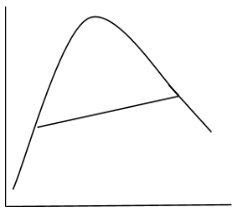
\includegraphics[scale=1]{grph.png}
		\caption{Density-Flow relation}
	\end{figure}
	In the graph, $x$-axis represents $\rho$ and $y$-axis represents flow $(q)$. Flow rate is a concave function in density and retains its maximum, the capacity at $\rho_c$. When $\rho_t$ is higher than the critical density, it is over-critical region and under-critical region otherwise [2].
	\subsubsection*{Flow}
	\addcontentsline{toc}{subsection}{\text{Flow}}
	Flow $q$ is the number of vehicles passing a reference point per unit of time, vehicles per hour [2]. Flow is obtained by the product of speed $v$ and density $\rho$.
	$$q = \rho v$$ Inverse of flow is headway $h$, which is the time that elapses between the $i$th vehicle passing a reference point in space and the $(i+1)$th vehicle. In traffic jam, $h$ approaches $\infty$.
	\subsection*{Kinematic wave traffic flow model}
	\addcontentsline{toc}{section}{\text{Kinematic wave traffic flow model}}
	Kinematic wave model is the simplest traffic flow model that reproduces the propagation of traffic waves. This model is made up of three components,
	\begin{itemize}
		\item[$\bullet$] Conservation laws
		\item[$\bullet$] Fundamental diagram
		\item[$\bullet$] Initial conditions
	\end{itemize}
	\subsubsection*{Conservation laws}
	\addcontentsline{toc}{subsection}{\text{Conservation laws}}
	These laws are the fundamental laws that vehicles are neither generated nor destroyed on a road section [3]. This can be described by an equation,
	$$\rho_t + q_x = 0$$ or
	$$\frac{\partial k}{\partial t} + \frac{\partial q}{\partial x} = 0$$
	\subsubsection*{Fundamental diagram}
	\addcontentsline{toc}{subsection}{\text{Fundamental diagram}}
	The fundamental diagram of the kinematic wave model appertains to traffic flow and density. Hence flow is the function of density.
	$$q = \phi (\rho)$$ This is the concave function as the diagram above [3].
	\subsubsection*{Initial conditions}
	\addcontentsline{toc}{subsection}{\text{Initial conditions}}
	For any model, initial conditions play a vital role in solving a problem. In traffic model, this takes two forms, initial value problems and boundary value problems. A boundary is defined to be $\rho (t, x)$, representing density as function of time and position. Because of the boundary values, aforementioned problems arise [3].
	\subsection*{Riemann's problem}
	\addcontentsline{toc}{section}{\text{Riemann's problem}}
	A Riemann problem, named after Bernhard Riemann, consists of an initial value problem composed of a conservation equation. It is highly useful in comprehending Eulers conservation equations because of properties namely, shocks and rarefaction waves appear as characteristics in the solution.
	
	\section*{Examples}
	\addcontentsline{toc}{chapter}{\textbf{Examples}}
	\subsection*{Google map density}
	\addcontentsline{toc}{section}{\text{Google map density}}
	The density flow is being inspired by Google's map constructions where the difference in density is represented by different colors; red, yellow and green representing high density, medium density and low density respectively.
	\section*{Learning outcomes}
	\addcontentsline{toc}{chapter}{\textbf{Learning outcomes}}
	%\subsection*{Our perspective}
	%\addcontentsline{toc}{section}{\text{Our perspective}}
	Here $a$ through $b$ is an interval that holds vehicles at some point of time [4].
	\begin{figure}[hbtp]
		\centering
		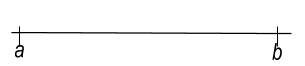
\includegraphics[scale=1]{interval.png}
		\caption{Vehicles in interval}
	\end{figure}
	Vehicles density function $\rho (x, t);$ $ x = $ position; $t = $ time.
	Number of vehicles between point a and b can be obtained by:
	$$q(t) = \int_a^b \rho (x, t)dx$$
	Traffic flow rate $(flux)$ is product of density $\rho$ and velocity $v.$
	$$q = \rho v$$
	Change of number of vehicles equals difference between inflow and outflow $q(a) - q(b).$
	$$\frac{d}{dt}q(t) = \int_a^b \rho_tdx = q(a) - q(b) = -\int_a^b q_xdx$$
	Equation holds for any choice of $a$ and $b.$
	$$\rho_t + (\rho v)_x = 0 \iff \rho_t + q_x = 0$$
	
	%\section*{Conclusion}
	%\addcontentsline{toc}{chapter}{\textbf{Conclusion}}
	
	%\bibliographystyle{IEEEtran}
	%\bibliography{bibo}
	\section*{Bibliography}
	\addcontentsline{toc}{chapter}{\textbf{Bibliography}}
	[1] William L Brogan, Modern Control Theory, 3rd ed. Pearson. 
	[2] Traffic Flow. \url{https://en.wikipedia.org/wiki/Traffic_flow}. 
	[3] Kinematic Wave Models of Network Vehicular Traffic. \url{http://www.its.uci.edu/~wjin/publications/jin2003dissertation.pdf} 
	[4] A Mathematical Introduction to Traffic Flow Theory \url{http://helper.ipam.ucla.edu/publications/tratut/tratut_12985.pdf}
\end{document}
